Most people have an intuition about what a substance is. A substance is just \textit{something}, like water, wood, butter or glass. A metal is a substance. The blood in your body is a substance. All of these are made up of atoms that form molecules in ways giving them very different properties. We know that a substance can exist in different phases, for example plasma, solid, liquid and gas \cite{ravndal2008statmech}, in which the same substance can behave very differently. Liquids and gases are often called fluids because they share the property that they do not have a fixed shape and are often easily deformed. The theory that describes how fluids behave is called fluid mechanics.\\
We start this chapter by discussing the Euler equations and the Navier-Stokes equations in section \ref{sec:theory_of_fluids_euler_navier}. They assume that the fluid can be described as a continuum, which turns out not to be true for what is called \textit{microflows}. The distinction between macroflows and microflows leads to what is called the breakdown of continuum, which is addressed in section \ref{sec:continuum_breakdown}. When studying microflows, one very important effect emerges; the slip velocity. It turns out that the slip velocity has major consequences for the permeability. This is discussed in section \ref{sec:slip_length}, before we in section \ref{sec:knudsen_number} introduce the Knudsen number which allows us to define different flow regimes in which we can categorize the validity of different fluid flow models.\\
We then define what a nanoporous media is before we in section \ref{sec:darcy_law} discuss Darcy's law, permeability and that we need to apply corrections to the permeability because of the effects of slip velocity.
\section{The Euler equations and the Navier-Stokes equations}
\label{sec:theory_of_fluids_euler_navier}
With the concept of continuum, we think that every point in space has well defined physical properties like temperature, density and momentum. In 1757, Euler published what's called the \textit{Euler equations} by applying conservation of mass, momentum and energy to a small volume element $\dm V$ of a fluid. They form a set of differential equations describing how the fluid velocity $\vec u$ field changes in time and space. The conservation laws can be written as
\begin{align}
	\dpart{\rho_m}{t} + \nabla\cdot (\rho_m\vec u) &= 0 \qquad \text{mass}\\
	\dpart{\rho_m \vec u}{t} + \nabla \cdot (\vec u \otimes (\rho_m\vec u)) + \nabla P &= 0\qquad \text{momentum}\\
	\dpart{E}{t} + \nabla\cdot (\vec u(E + p)) &= 0\qquad \text{energy},
\end{align}
where $\rho_m$ is the mass density, $\vec u(\vec r, t)$ is the velocity field, $E$ is the total energy per unit volume, $p$ is the pressure field and $\otimes$ is the tensor product. These can be combined to one vector equation, but the connection to conservation laws is more clear when they are separated. In the original paper, Euler only derived the first two equations, but the full set is usually referred to as the Euler equations. They describe the motion of fluids with negligible viscosity, which is a decent approximation for many fluids.\\
About 80 years later, in the 1840s, Sir George Stokes published the Navier-Stokes equations (NSE) which can be seen as an extension of the Euler equations where effects caused by the viscosity of the fluid are included \cite{batchelor2000introduction}. The Navier-Stokes equations for an incompressible fluid can be written as one vector equation
\begin{align}
	\label{eq:nse}
	\rho_m \frac{D\vec u}{ Dt} = \rho_m \vec F - \nabla p + \mu\nabla^2\vec u + \mu\nabla(\nabla\cdot \vec u)
\end{align}
where $\vec F$ is an external force (i.e. gravity or an electrostatic field), $\mu$ is the viscosity and $D/Dt$ is the material derivative defined as
\begin{align}
	\frac{D}{Dt} = \dpart{}{t} + \vec u\cdot \nabla.
\end{align}
The NSE has quite a few interesting analytically solvable solutions, but for most real systems, the geometry confining the fluid is so complex that it is usually solved on computers. When solving the NSE, one has to provide boundary conditions to get a unique solution for the system. Usually, one applies no-slip boundary conditions, i.e. that the fluid velocity is zero at the container walls. It turns out that for real fluids, this is not always the case. In section \ref{sec:slip_length} we discuss the effects of slip velocity and how this affects the flow properties of the fluid. 
\section{Macroflows and microflows}
\label{sec:theory_of_fluids_microflows}
When we solve the equations governing our fluid flow, we add boundary conditions defining the geometry of our system. In the 1990s H. Bau and J. Zemel (University of Pennsylvania) performed experiments on microchannel flow in which they found clear deviations from what was expected from the theory\cite{karniadakis2005microflows}. It is useful to introduce the terms \textit{microflows} for flow in geometries where the distance between the channel walls is of order micrometer or smaller, and \textit{macroflows} for larger systems (milimeter and above). Flow at microscales differ from macroscales because of effects that can be classified into four groups
\begin{itemize}
\item noncontinuum effects,
\item surface-dominated effects,
\item low Reynolds number effects, and
\item multiscale and multiphysics effects.
\end{itemize}
In this thesis, we focus on the noncontinuum effects which are briefly discussed in section \ref{sec:continuum_breakdown}, and the surface-dominated effects as the slip condition described in section \ref{sec:slip_length}. See \cite{karniadakis2005microflows} for details about the effects of low Reynolds number, multiscale and multiphysics. 

\section{The breakdown of continuum}
\label{sec:continuum_breakdown}
A fundamental assumption in the derivation of the NSE is that the space is continuous. But we know that in reality, the mass of the fluid is concentrated in the center of the atoms, but we often assume that the mass is uniformly distributed in the volume element of which the conservations laws are applied on. This is known as the \textit{continuum hypothesis} and is invalid when the \textit{mean free path} $\lambda$, the average distance a particle moves between collisions, becomes large compared to some characteristic length $L$ in the system, i.e. the diameter of a channel\cite{karniadakis2005microflows}. This property is quantified through the \textit{Knudsen number}
\begin{align}
	\text{Kn} = \frac{\lambda}{L}.
\end{align}
From the kinetic theory we can calculate the mean free path (this is done in section \ref{sec:mean_free_path_calculation})
\begin{align}
	\lambda = \frac{m}{\sqrt 2 \pi d \rho_n} = \frac{k_B T}{\sqrt 2 \pi d^2 P},
\end{align}
where $\rho_n$ is the number density and $m$ and $d$ are the mass and diameter of the particles. By using the ideal gas law $P = \rho_n k_BT$, we can replace the density with the pressure $P$ and the temperature $T$. Here $k_B$ is Boltzmann's constant. For Knudsen numbers smaller than $10^{-2}$, the continuum hypthosis is valid and we can apply the Navier-Stokes equations\cite{karniadakis2005microflows}. It turns out that the Knudsen number is very useful, so we will get back to it in section \ref{sec:knudsen_number}.
\section{Slip velocity}
\label{sec:slip_length}
As already mentioned, the NSE need boundary conditions of the velocity field defining the geometry of which the fluid is confined in. The simplest boundary condition is the no-slip condition where
\begin{align}
	\vec u(\vec r; t) = 0 \qquad \vec r \in \partial\Omega
\end{align}
where $\partial\Omega$ defines the boundary domain. The history of the no-slip condition was studied by Day\cite{day1990no}, based on the work of Stokes in the 19th century. Stokes compared theoretical results to experiments for pendulums of different kinds and concluded that
\begin{aquote}{Stokes, 1901}
	I shall assume, therefore, as the conditions to be satisfied at the boundaries of the fluid, that the velocity of a fluid particle shall be the same, both in magnitude and direction, as that of the solid particle with which it is in contact. The agreement of the results thus obtained with observation will presently appear to be highly satisfactory.
\end{aquote}
In Day's detailed study of the no-slip condition, he says
\begin{aquote}{Day, 1990}
	Looking back, it appears that the acceptance of a more general no-slip condition was prolonged because of experimental shortcomings, not because of a lack of the \'appropriate\' theoretical solutions to fluid flow problems.
\end{aquote}
In other words, the theoretical framework that existed already in the time of Stokes were complete enough to include both slip and no-slip solutions. In fact, Maxwell predicted slip velocity in a paper already in 1867\cite{maxwell1879stresses}, but the experiments the next 50 years seemed to more or less confirm the no-slip condition.\\
But 

 Klinkenberg also has a nice argument that supports the slip velocity
\begin{aquote}{L.J. Klinkenberg, 1941}
Consider a layer adjacent to the wall which is thinner than the mean free path $\lambda$ of the gas molecules, so that practically a molecule does not collide with other molecules present in this layer. At a given moment half of the gas molecules in this layer will have a component of velocity moving towards the wall; the other half in the opposite direction. The molecules moving towards the wall have had their last collision somewhere in the flowing mass, and, therefore, will have an average velocity component in the direction of flow different from zero. A part of this average velocity component will be lost in colliding with the wall. Even if the molecules lose it entirely, then still the average velocity component in the direction of flow of all the molecules contained in the layer will amount to half of the average velocity component of the molecules moving towards the wall. The gas in the layer, therefore, will have a finite rate of flow.
\end{aquote}
It is convenient to introduce the concept of \textit{slip length} $l_s$ to be able to quantify the slip velocity. Slip length is defined as the distance into the wall we would have to extrapolate a velocity profile for it to reach zero value, see figure \ref{fig:slip_length}.
\begin{figure}[h]
\begin{center}
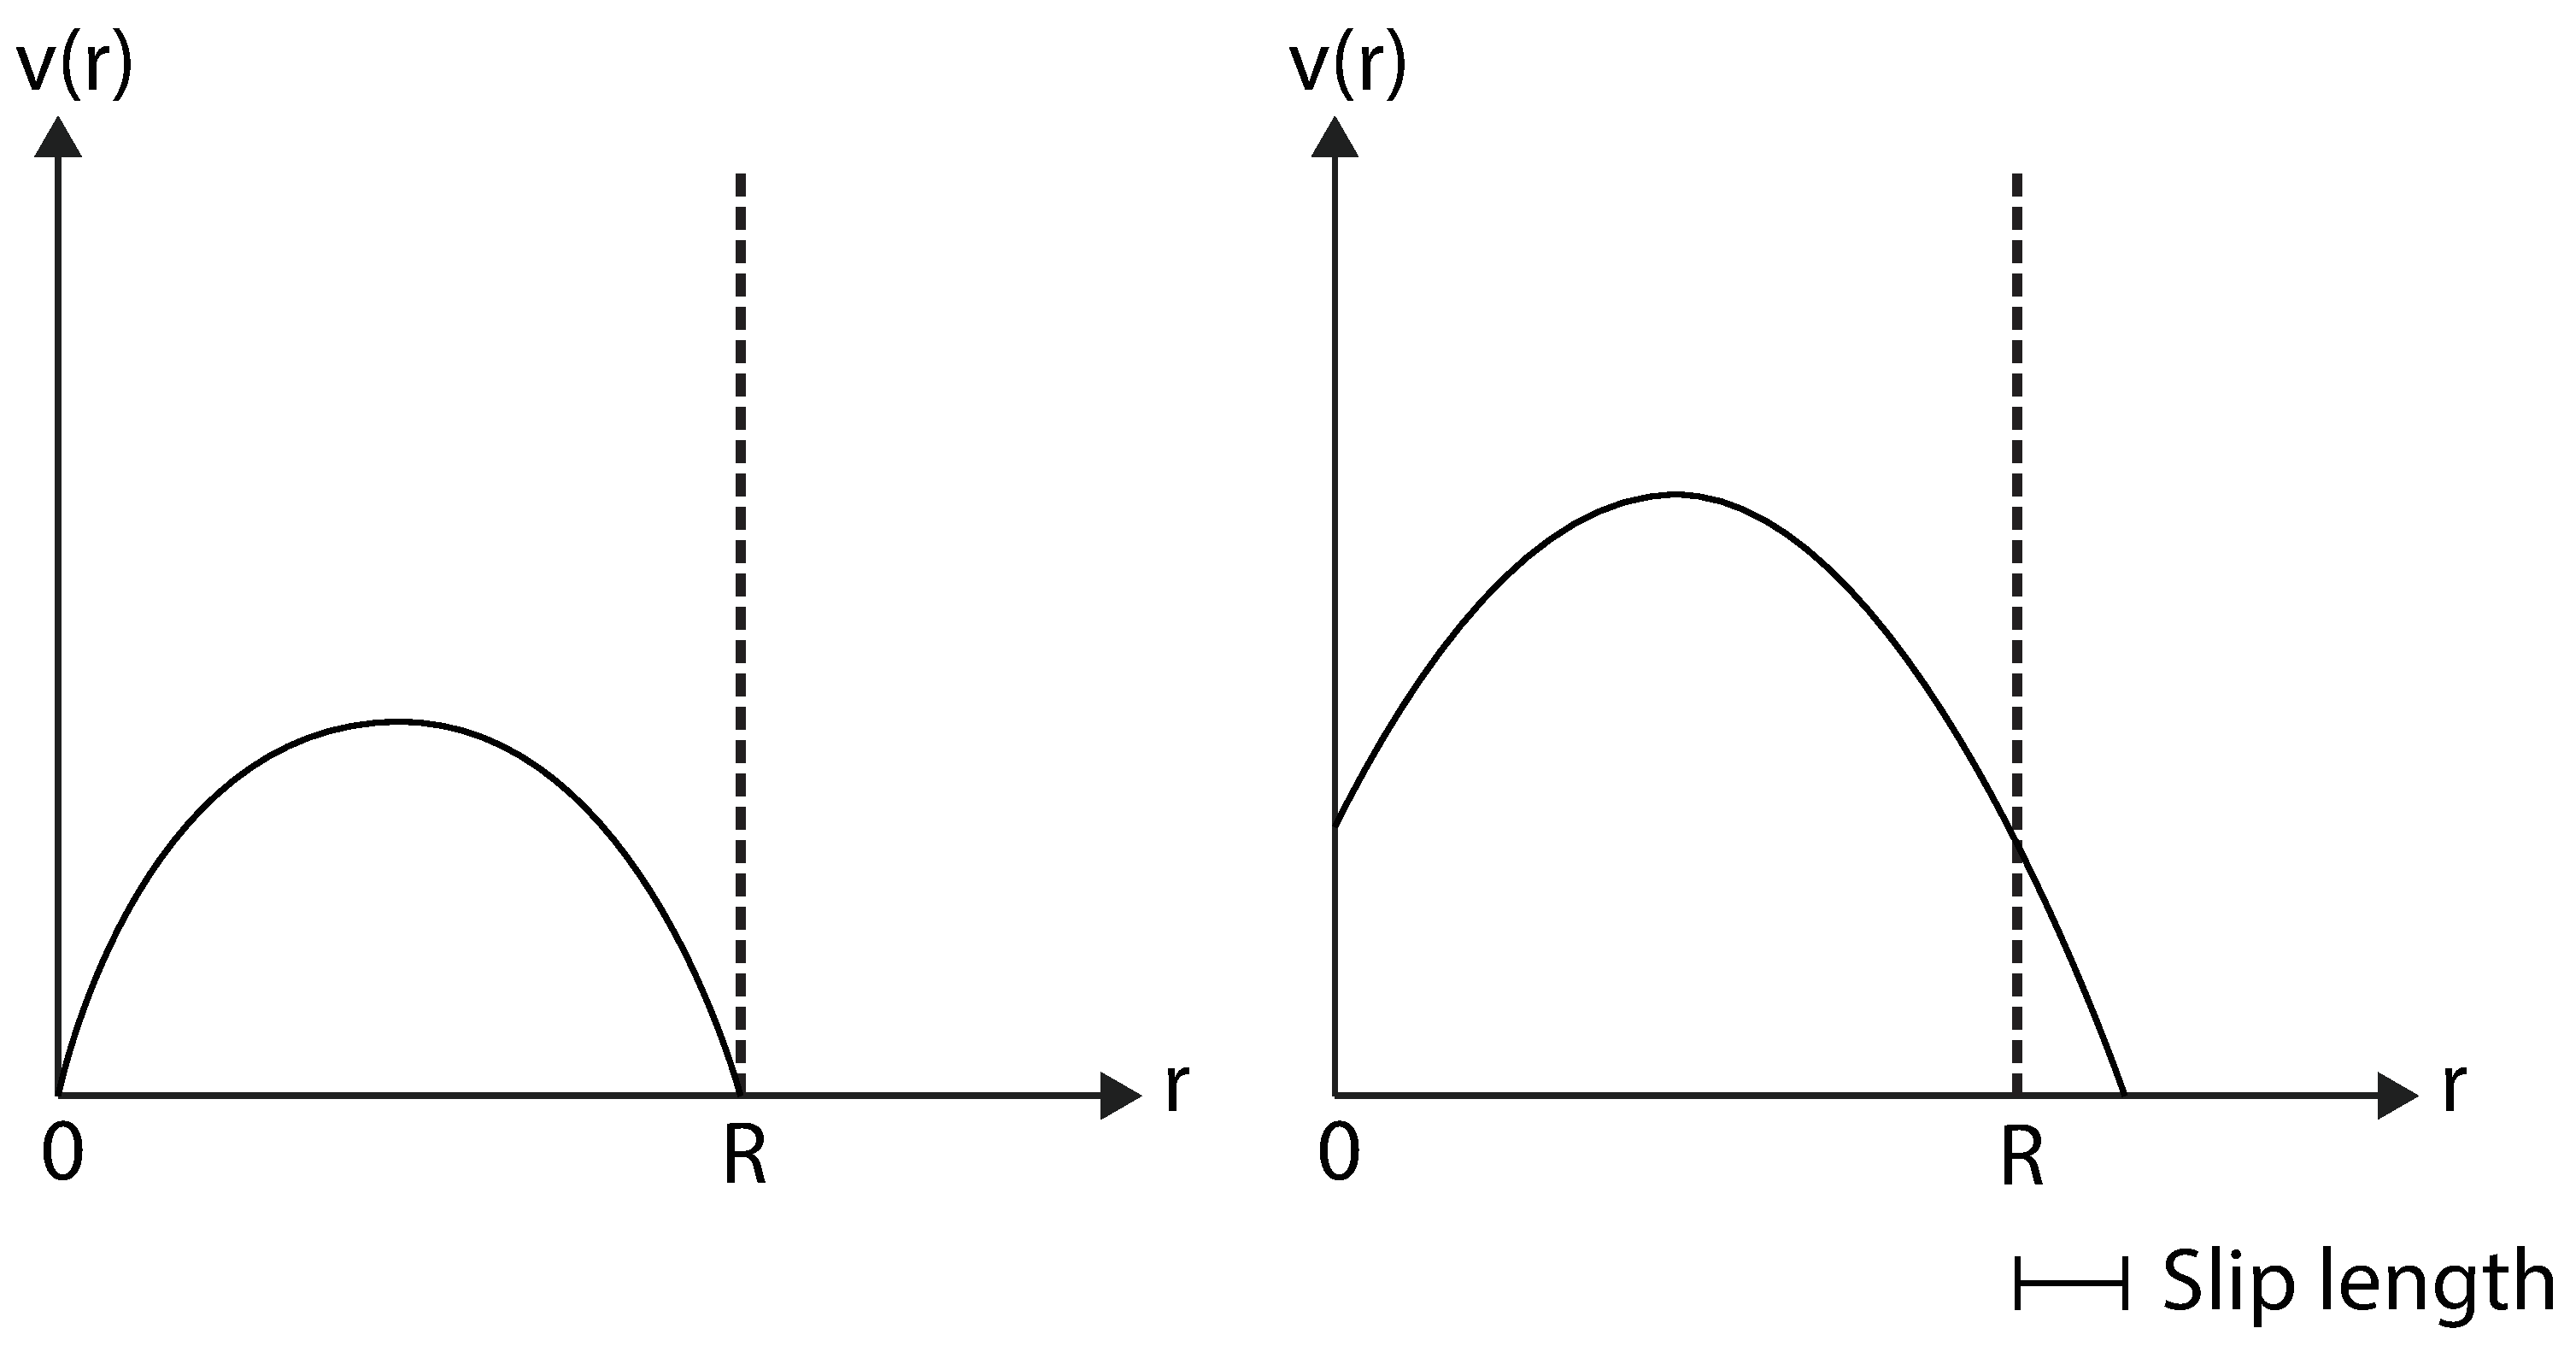
\includegraphics[width=\textwidth, trim=0cm 0cm 0cm 0cm, clip]{DSMC/figures/slip_length.eps}
\end{center}
\caption{Slip length is the distance into the wall we would have to extrapolate a velocity profile for it to reach zero value. We have the no-slip condition on the left, where the slip length is zero whereas we have a non-zero slip length on the right.}
\label{fig:slip_length}
\end{figure}
Maxwell theory predicts the following relation between the slip length and the mean free path
\begin{align}
	\label{eq:noslip_sliplength}
	l_s = \alpha \lambda,
\end{align}
where $\alpha\approx 1.15$ is the slip coefficient \cite{morris1992slip}. The effects of slip velocity become more apparent when the channel diameter is of the same order as the mean free path. By introducing the dimensionless slip length
\begin{align}
	l_s^* = \frac{l_s}{ L} = \alpha \frac{\lambda }{ L} = \alpha \text{Kn},
\end{align}
we see that the ratio of the slip length to the channel diameter is proportional to the Knudsen number. The actual slip velocity (the average velocity of the molecules right next to the wall) can be written as
\begin{align}
	\label{eq:linear_slip_velocity}
	v_{\text{wall}} = \alpha\lambda\frac{\dm v}{\dm n},
\end{align}
where $n$ is the direction normal on the wall\cite{klinkenberg1941permeability}. We call this a \textit{first order} slip model since it is contains only the first derivative of the velocity. Higher order models exists and give corrections that are important in nanoporous media (which is defined in section \ref{sec:nanoporous_media}) where the channels that contribute to flow are of nanometer scale.

\section{Knudsen number}
\label{sec:knudsen_number}
To get an idea of the length scales where the Knudsen number is about unity, the mean free path for helium at $T=$\unit{273}{\kelvin} and $P=1$ atm is\cite{lillestol2001generell} 
\begin{align}
	\label{eq:helium_mfp}
	\lambda_{\text{He}} = \unit{0.17}{\micro\meter} = \unit{170}{\nano\meter}.
\end{align}
This means that for systems where the channels have diameter of a few hundred nanometers, the Knudsen number is around unity, and the continuum hypothesis is invalid. 

\section{Atomic models}
\label{sec:theory_of_fluids_atomic_models}
For systems where the continuum hypothesis is invalid, we need other models describing the behaviour of the particles in our system. The first idea that might pop our minds might be to study the system at the atomic level. The physical set of rules that are controlling the atoms is of course quantum mechanics. The equations of motion and hence the dynamics of an atomic system can in principle be calculated directly from quantum mechanics by solving Schr\"{o}dinger's equation with perturbation theory. Since this requires calculating the wave function of every atom with complex atomic interactions, the size of the system needs to be very small with today's computers. An alternative, popular approach is to use a parameterized potential $U(\vec r^N)$ ($\vec r^N$ being the positions of all atoms), and calculate the forces through the gradient of $U$. Newton's equations of motion is then integrated and the dynamics of the system are determined in a classical, deterministic way where important effects from quantum mechanics can be embedded in the potential. This method is called \textit{Molecular Dynamics} and is studied in chapter \ref{chap:md}. Molecular Dynamics is orders of magnitudes faster than models solving Schr\"{o}dinger's equation, but it still needs a detailed describtion of the dynamics of every atom in the system. For many problems, this information is redundant because what's really important is the statistical properties of the system.

 It is convenient to classify different flow regimes 
\section{Flow regimes}

\todo{Discuss flow regimes}
\section{Nanoporous media}
\label{sec:nanoporous_media}
A porous medium is a material with pores and channels (the pore network) available for fluids. See figure \ref{fig:history_porous_media}. 
\missingfigure{Make a sketch of a porous medium.}